In the homogeneous system, we assume zero friction and horizontal bathymetry. Our SWE system then becomes

$$
\renewcommand*{\arraystretch}{1.5}\begin{bmatrix}
    
    h_t + v h_x + h v_x \\
    v_t + g h_x + v v_x
\end{bmatrix} = \begin{bmatrix}
    0 \\
    0
\end{bmatrix}.
$$
\ \\\\
\noindent We impose periodic boundary conditions on $h$ and $v$ with initial conditions

$$
h(x, 0) = 2 + \sin{\left( \frac{\pi x}{100} \right)}, \quad v(x, 0) = 0
$$

\noindent where $x \in [0, 200]$ and $t \in [0, 15]$. We use a neural network with three hidden layers with 20 neurons 
each and Glorot weight initialization \cite{glorot2010understanding}. After training the network with a learning rate
$\alpha = 0.001$ over 50000 Adam iterations and 12000 L-BFGS iterations, we obtain a mean residual value

$$
R(\Omega) = MSE_f = 0.006090
$$

\noindent over a randomly sampled subset $\Omega$ of the computational domain. The results of this computation are shown 
in Figure \ref{fig:homogeneous_swe_solution}.

\begin{figure}[h]
    \centering
    \begin{subfigure}[b]{0.45\textwidth}
        \centering
        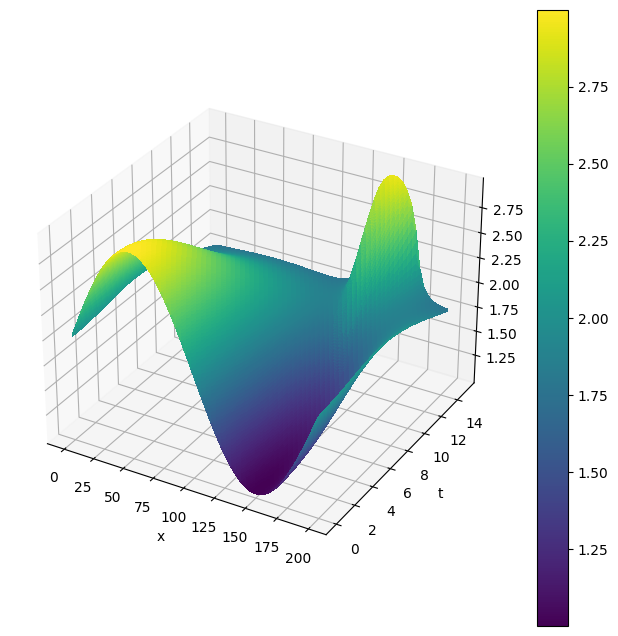
\includegraphics[width=\textwidth]{images/homogeneous_swe_pseudospectral_height.png}
        \caption{Reference wave height}
        \label{fig:homogeneous_pseudospectral_swe_height}
    \end{subfigure}
    \hfill
    \begin{subfigure}[b]{0.45\textwidth}
        \centering
        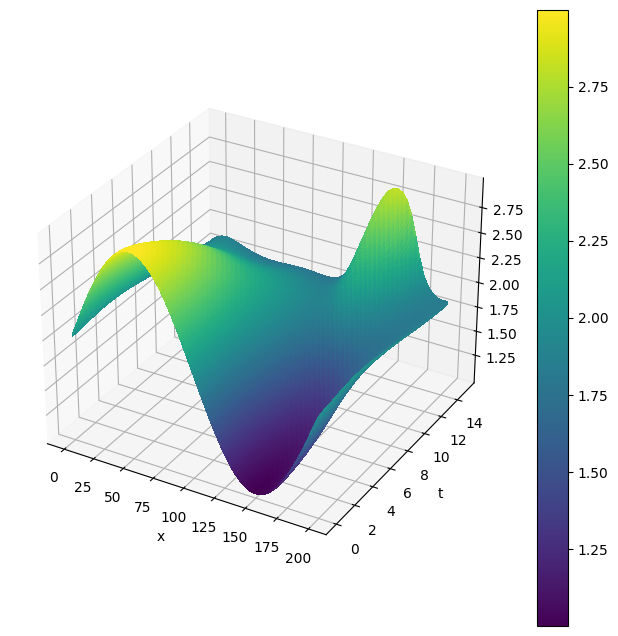
\includegraphics[width=\textwidth]{images/homogeneous_swe_pinn_height.png}
        \caption{PINN wave height}
        \label{fig:homogeneous_pinn_swe_height}
    \end{subfigure}
    \begin{subfigure}[b]{0.45\textwidth}
        \centering
        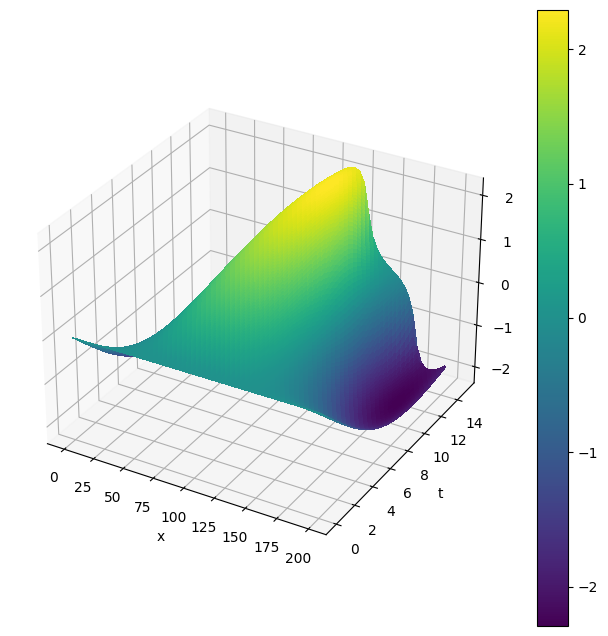
\includegraphics[width=\textwidth]{images/homogeneous_swe_pseudospectral_velocity.png}
        \caption{Reference wave velocity}
        \label{fig:homogeneous_pseudospectral_swe_velocity}
    \end{subfigure}
    \hfill
    \begin{subfigure}[b]{0.45\textwidth}
        \centering
        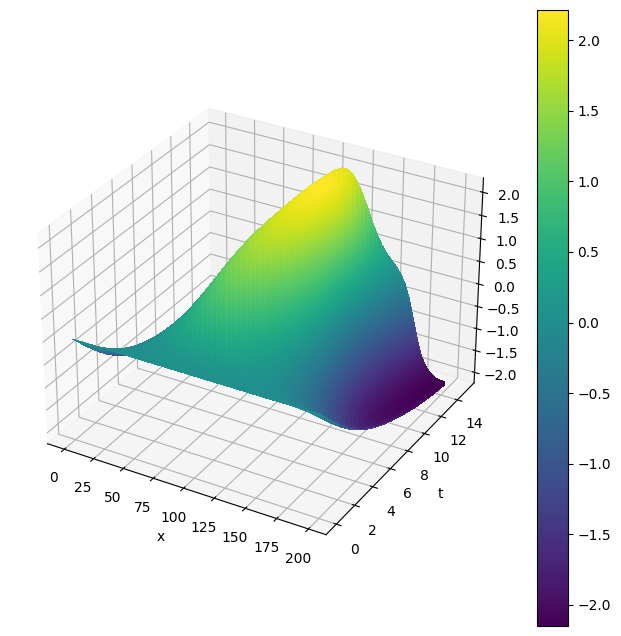
\includegraphics[width=\textwidth]{images/homogeneous_swe_pinn_velocity.png}
        \caption{PINN wave velocity}
        \label{fig:homogeneous_pinn_swe_velocity}
    \end{subfigure}
    \caption{Pseudospectral and PINN solutions for the homogeneous SWE system.}
    \label{fig:homogeneous_swe_solution}
\end{figure}

As we might expect from the small PDE residual value, we observe good visual agreement between pseudospectral and PINN 
solutions.